\documentclass[12pt]{article} 
\usepackage{graphicx} 
\usepackage{titlesec}

% Replace `letterpaper' with `a4paper' for UK/EU standard size
\usepackage[a4paper,top=2cm,bottom=2cm,left=3cm,right=3cm,marginparwidth=1.75cm]{geometry}

% Useful packages
\usepackage{amsmath}
\usepackage{graphicx}
\usepackage{tabularx} % Include the tabularx package
\usepackage{hyperref}
\usepackage{caption}
\usepackage{subcaption}
\usepackage{caption}
\usepackage{subcaption}
\usepackage{placeins}
\usepackage{amssymb} % This package defines \mathbb
\usepackage{booktabs} % For professional looking tables
\usepackage{amsfonts}

% Center section headings
\titleformat{\section}
  {\normalfont\Large\bfseries}
  {\thesection}
  {1em}
  {}
 

\begin{document}

\begin{titlepage}
\centering
\vspace{0.5cm}
{\Huge\bfseries Mixture of Experts\par}

\vspace{0.5cm} % Adds vertical space
{\Large SAiDL 2024 Assignment}

\vspace{1.5cm}
{\Large Sasmit Datta}
\end{titlepage}

%%%%%%%%%%%%%%%%%%%%%%%%%%%%%%%%%%%%%%%%%%%%%%%
\section{Introduction}
Mixture of Experts (MoE) is a machine learning framework designed to integrate multiple models or "experts" which handle different tasks in a parallel fashion for improved prediction performance. In the context of this report the MoE layer is an assortment of MLPs. 

I developed two baseline models: one consisting of stacked two LSTMs with an intermediate MLP "expert" layer, and another one with an MoE layer. 

My primary focus was on exploring various gating strategies for these networks, including \textbf{top-k gating}, \textbf{top-k mask}, \textbf{noisy top-k}, and the incorporation of \textbf{importance} and \textbf{load} losses, to optimize the allocation of tokens among experts. I also plotted router distributions for these different strategies.
%%%%%%%%%%%%%%%%%%%%%%%%%%%%%%%%%%%%%%%%%%%%%%%
\section{Mixture of Experts}
The mathematical formulation of the MoE model is given by:
\begin{equation}
\mathbf{y} = \sum_{i=1}^{N} G_i(\mathbf{x}) \cdot E_i(\mathbf{x})
\end{equation}
where $\mathbf{y}$ is the output, $\mathbf{x}$ is the vector input, $N$ is the number of experts, $G_i(\mathbf{x})$ is the gating function output for the $i$-th expert, determining its contribution weight, and $E_i(\mathbf{x})$ is the output of the $i$-th expert for input $\mathbf{x}$.
\subsection{Architecture of Expert}
For models of both datasets, the expert is a simple MLP with one \textbf{hidden layer} of \textbf{128 dimensions}. A \textbf{ReLU activation} is used before the input enters the hidden layer and \textbf{dropout} with $\boldsymbol{p=0.5}$ is used at the end.

%%%%%%%%%%%%%%%%%%%%%%%%%%%%%%%%%%%%%%%%%%%%%%%
\section{Model Variations}
For each dataset I trained six different models, a baseline LSTM, and 6 LSTM's with an intermediate MoE layer with different gating strategies and losses. The models with MoE have same architecture for each dataset described in their respective sections. The gating strategies and losses are explained in Section \ref{gating}.
\begin{table}[h]
  \centering
  \begin{tabular}{lcc}
  \hline
  \textbf{Model Name} & \textbf{About}                        \\ \hline
  LSTM Baseline       &Two LSTMs with intermediate expert layer                       \\
  MoE Naive           &Two LSTMs with MoE layer with Naive Top-K Gating                       \\
  MoE Mask            &Two LSTMs with MoE layer with Top-K Mask Gating                         \\
  MoE Noisy TopK      &Two LSTMs with MoE layer with Noisy Top-K Gating                      \\
  MoE Importance      &Two LSTMs with MoE layer with Top-K Mask and $L_{\text{importance}}$                        \\
  MoE Load            &Two LSTMs with Moe layer with Noisy Top-K Gating and $L_{\text{Load}}$ \\ \hline
  \end{tabular}
  \caption{Model Performance on CoNLL dataset}
  \label{tab:models}
  \end{table}

%%%%%%%%%%%%%%%%%%%%%%%%%%%%%%%%%%%%%%%%%%%%%%%
\section{CoNLL-2003 Dataset}
The CoNLL-2003 dataset is a collection of annotated texts that is widely used for training and evaluating machine learning models on named entity recognition (NER) tasks.

It includes a set of tags for named entity recognition that denote the beginning (B) and inside (I) of named entities, as well as tags for non-entity segments (O). The entity types covered include persons (PER), organizations (ORG), locations (LOC), and miscellaneous entities (MISC), each of which is prefixed by either B- or I- to indicate the position of the token within the entity.
\subsection{Preprocessing}
For preprocessing the CoNLL-2003 dataset, I created a unified vocabulary from all tokens, reduced it to match \textbf{GloVe 6B 50-dimensional} embeddings. This process involved removing non-GloVe tokens, adding special \textbf{padding} and \textbf{unknown} tokens, resulting in a pruned vocabulary. Token-to-index mappings were established, followed by the creation of an embedding matrix populated with GloVe vectors for each token. A \textbf{vector of zeros} was used for \textbf{padding} token and while the \textbf{unknown} token had the default \textbf{GloVe} $<$unk$>$ token assigned to it.
\subsection{Pipeline}
The tokenizer maps the words in a given data point to their corresponding indexes and post-pads the given sequence to a \textbf{maximum length} of \textbf{128} with 0's (index of padding token). The \textbf{NER tags} are already in their numerical form and hence just \textbf{padded with -100} for the cross entropy loss to ignore them.

\subsection{Training}
For the base model, I used an expert layer sandwiched between two \textbf{bidirectional LSTM} layers with \textbf{hidden dimension 128} and a linear layer as a head to map the outputs to \textbf{9 dimensions} (number of NER tags).

For the MoE models, I just replace the single expert layer with a mixture of experts layer with \textbf{8 experts} and $\boldsymbol{k=2}$. I use a \textbf{batch size} of \textbf{32} and train all the models for \textbf{10 epochs} each.

\subsection{Results}

\begin{table}[h]
  \centering
  \begin{tabular}{lcc}
  \hline
  \textbf{Model Name} & \textbf{Validation Accuracy (\%)} & \textbf{Validation Loss} \\ \hline
  LSTM Baseline       &97.08                         &0.1179                    \\
  MoE Naive           &97.08                         &0.1142                    \\
  MoE Mask            &97.26                         &0.1173                    \\
  MoE Noisy TopK      &97.31                         &0.1087                    \\
  MoE Importance      &97.40                         &0.1095                    \\
  MoE Load            &97.30                         &0.1133                    \\ \hline
  \end{tabular}
  \caption{Model Performance on CoNLL dataset}
  \label{tab:performance_conll}
  \end{table}
  
\begin{figure}[h]
  \centering
  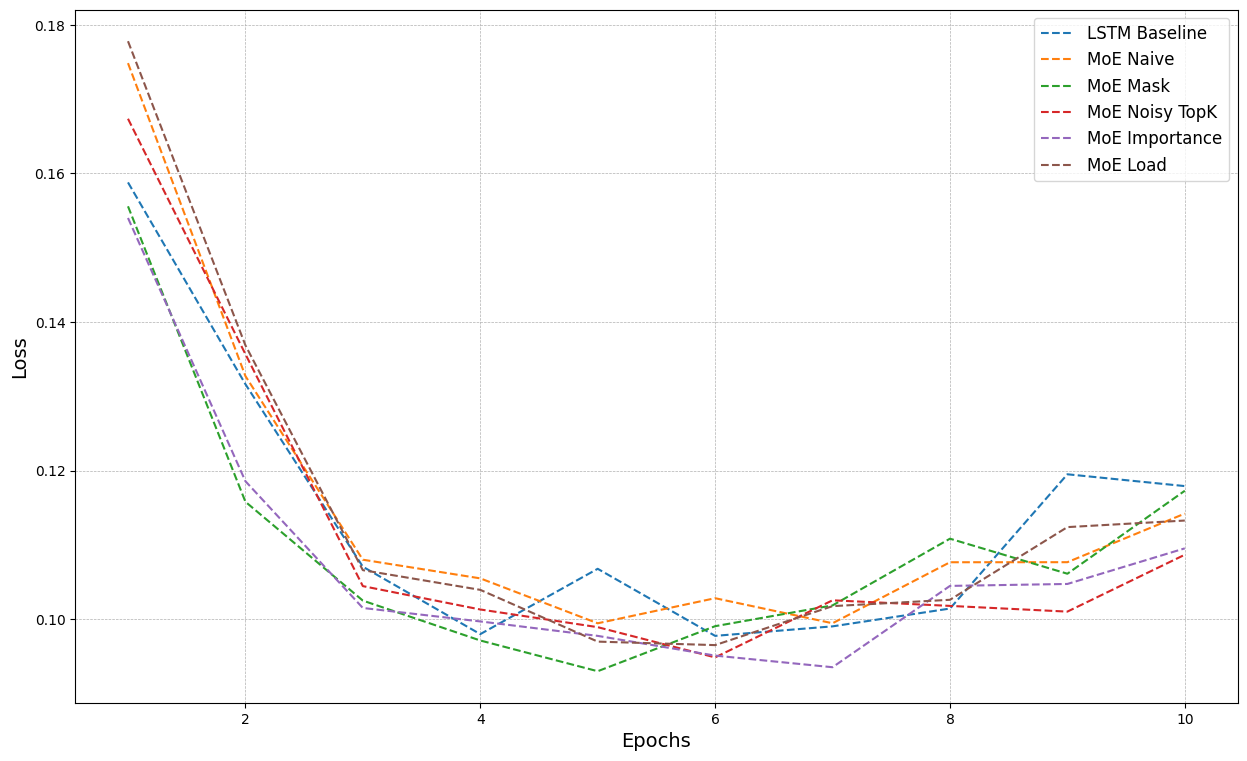
\includegraphics[width=1\linewidth]{report_images/conll/loss.png}
  \caption{\label{fig: conll_losses}Loss Plots CoNLL}
  \end{figure}
  \noindent



%%%%%%%%%%%%%%%%%%%%%%%%%%%%%%%%%%%%%%%%%%%%%%%
\section{SQuAD 1.1 Dataset}
The SQuAD 1.1 dataset is a collection of over 100,000 questions derived from approximately 500 Wikipedia articles, designed for training and evaluating question answering models. 

Each entry in the dataset features a context (a text passage from an article), a question generated by human annotators based on the context, an answer to the question, and the starting position of the answer within the context. This structure supports extractive question answering, where models are tasked with identifying the exact span of text that answers the question.

\subsection{Preprocessing}
The preprocessing of the SQuAD 1.1 dataset involved \textbf{transforming} raw JSON data into structured \textbf{pandas DataFrames} by extracting contexts, questions, answers, and answer start positions. 

Texts were tokenized using regex, maintaining punctuation as distinct tokens. Entries exceeding predefined \textbf{context} and \textbf{question} \textbf{length} of \textbf{256} tokens were filtered out. \textbf{Character indices} for \textbf{answer starts} were \textbf{converted into token indices} to align with the tokenized contexts. 

A vocabulary was compiled from the tokenized texts, pruned to match \textbf{GloVe 6B 50d embeddings}, and \textbf{padding} and \textbf{unknown} tokens. 

\subsection{Pipeline}
Like CoNLL, the tokenizer maps the words of a given context and question to their corresponding indexes and post-pads the two separate sequences with 0's to \textbf{maximum length} of \textbf{256}. Then with the help of the start index and the length of answer text, the end index of the answer is calculated.

\subsection{Training}
Like CoNLL, for the base model, I use an expert layer sandwiched between two \textbf{bidirectional LSTM} layers with \textbf{hidden dimension 128}. Unlike the CoNLL model, I use a head which maps the outputs to a \textbf{single dimension} as the model has to predict the position in the context where answer starts and ends. 

I \textbf{concatenate} the \textbf{context and question} before passing it through the embedding layer, making the total input sequence length to 512. I \textbf{split the output} to get the \textbf{answer start} and the \textbf{answer end logits}. Essentially, I convert this into a classification task with number of classes equal to the sequence length of the context.

For the MoE models, I just replace the single expert layer with a mixture of experts layer with \textbf{8 experts} and $\boldsymbol{k=2}$. I use a \textbf{batch size} of \textbf{32} and train all the models for \textbf{5 epochs} each.

\subsection{Results}

\begin{table}[h]
  \centering
  \begin{tabular}{lcc}
  \hline
  \textbf{Model Name} & \textbf{Validation Accuracy (\%)} & \textbf{Validation Loss} \\ \hline
  LSTM Baseline       &11.45                         &8.770                    \\
  MoE Naive           &11.62                         &8.710                    \\
  MoE Mask            &11.47                         &8.766                    \\
  MoE Noisy TopK      &11.40                         &8.717                    \\
  MoE Importance      &11.46                         &8.794                    \\
  MoE Load            &11.76                         &8.710                    \\ \hline
  \end{tabular}
  \caption{Model Performance on SQuAD dataset}
  \label{tab:performance_squad}
  \end{table}
  
\begin{figure}[h]
  \centering
  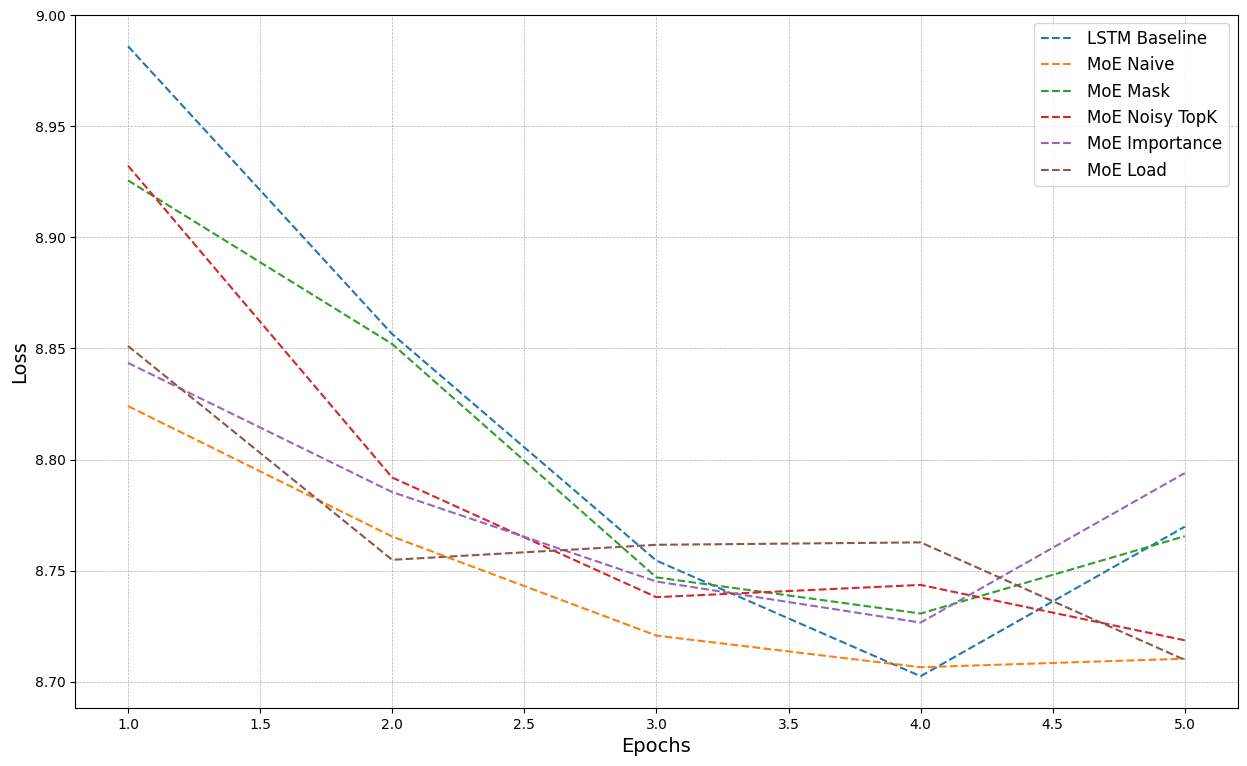
\includegraphics[width=1\linewidth]{report_images/squad/loss.png}
  \caption{\label{fig: squad_losses}Loss Plots SQuAD}
  \end{figure}
  \noindent


%%%%%%%%%%%%%%%%%%%%%%%%%%%%%%%%%%%%%%%%%%%%%%%
\section{Gating Strategies and Losses} \label{gating}

\subsection{Naive Top-K Gating}
\begin{equation}
G(\mathbf{x}) = \text{Softmax}(\mathbf{x\cdot W}_g)\odot \text{TopK}(\mathbf{x},k)
\end{equation}
where,
\begin{equation}
\text{TopK}(\mathbf{v}, k)_i = 
\begin{cases} 
1 & \text{if } v_i \text{ is in the top } k \text{ elements of } v. \\
0 & \text{otherwise}.
\end{cases}
\end{equation}
$\mathbf{W}_g$ is the trainable weight matrix, $k$ is the number of experts per token and  $\mathbf{x}$ is the input.

Essentially what this gating function does is naively multiplies the weights assigned by the router to the outputs of the top-k experts and adds them up. 

\begin{figure}[h]
\centering
\begin{subfigure}{.5\textwidth}
  \centering
  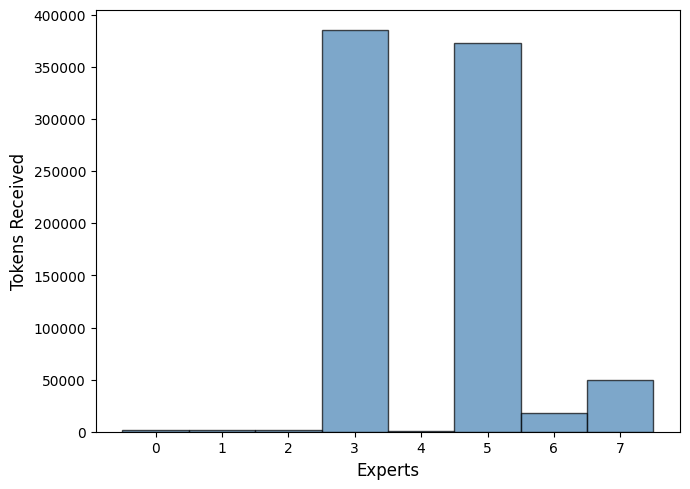
\includegraphics[width=1\linewidth]{report_images/conll/naive.png}
  \caption{CoNLL-2003}
  \label{fig:naive_conll}
\end{subfigure}%
\begin{subfigure}{.5\textwidth}
  \centering
  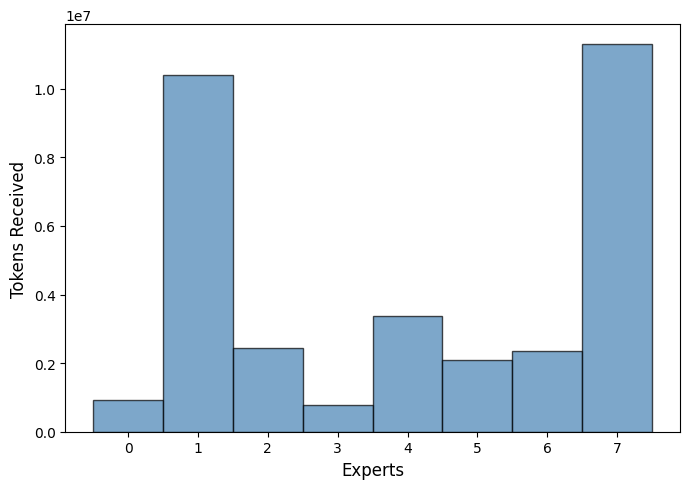
\includegraphics[width=1\linewidth]{report_images/squad/naive.png}
  \caption{SQuAD 1.1}
  \label{fig:naive_squad}
\end{subfigure}
\caption{Naive Top-K Gating Expert Distributions}
\label{fig:naive}
\end{figure}
\FloatBarrier
\noindent
In Fig \ref{fig:naive} we can see that the distribution of the model trained on the SQuAD dataset is more skewed. Since the model performs quite well on CoNLL dataset (Fig \ref{fig:naive_conll}) it might suggest that two experts are sufficient for the task at hand. Plus, model performance on SQuAD is terrible, hence the router might be trying its best to distribute tokens for more parameter usage.


\subsection{Top-K Mask Gating}
Instead naively multiplying the top-k weights above with the expert outputs, we first normalize them.
$$
G_{\sigma}(\mathbf{x}) = \text{Softmax}(\mathbf{x\cdot W}_g)\cdot 
$$
Therefore,
\begin{equation}
G(\mathbf{x})_i = \frac{G_{\sigma}(\mathbf{x})_i\text{TopK}(\mathbf{v}, k)_i}{\sum_{j=1}^nG_{\sigma}(\mathbf{x})_j\text{TopK}(\mathbf{v}, k)_j}
\end{equation}
where $n$ is the dimensions of our vector.

For the model being trained on CoNLL dataset, the router still continued to focus on just two experts but unlike before, the model trained on SQuAD only had its focus on four (Fig \ref{fig:mask}). Normalization causes the router to narrow in only certain experts, not utilising the model's full potential which is not ideal.

\begin{figure}[h]
\centering
\begin{subfigure}{.5\textwidth}
  \centering
  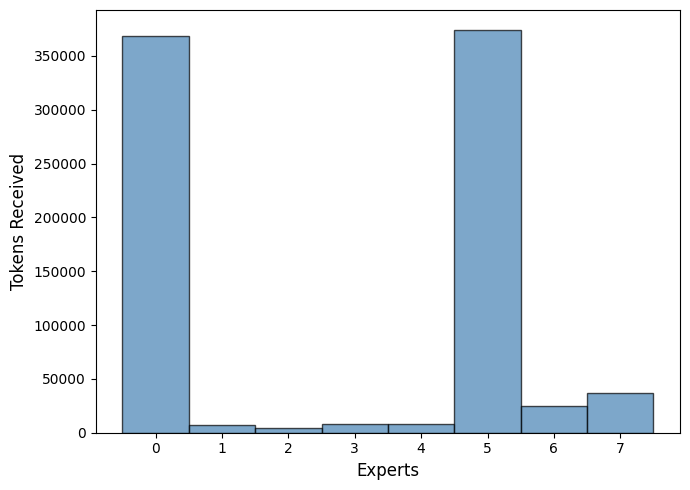
\includegraphics[width=1\linewidth]{report_images/conll/top_k_mask.png}
  \caption{CoNLL-2003}
  \label{fig:mask_conll}
\end{subfigure}%
\begin{subfigure}{.5\textwidth}
  \centering
  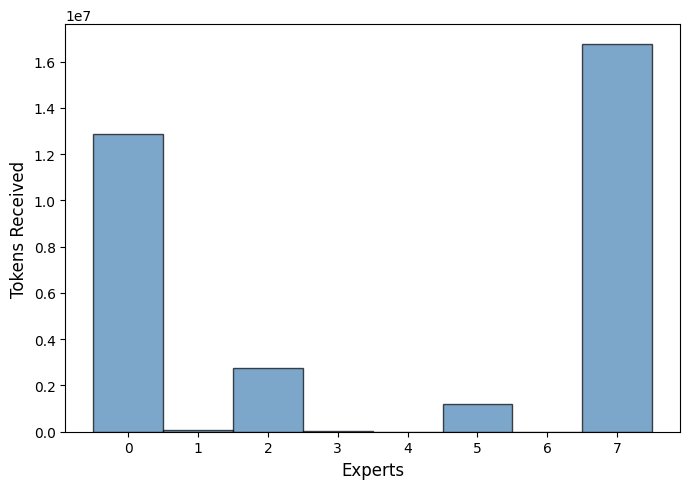
\includegraphics[width=1\linewidth]{report_images/squad/top_k_mask.png}
  \caption{SQuAD 1.1}
  \label{fig:mask_squad}
\end{subfigure}
\caption{Top-K Mask Gating Expert Distributions}
\label{fig:mask}
\end{figure}
\FloatBarrier




\subsection{Noisy Top-K Gating}
Unlike standard Top-K gating, which deterministically selects the $k$ experts with the highest gate values, noisy top-k adds randomness to the gating procedure, potentially allowing for exploration of less frequently chosen experts.
\begin{equation}
G(\mathbf{x}) = \text{Softmax}(\text{KeepTopK}(H(\mathbf{x}), k))
\end{equation}
where
\begin{equation}
H(\mathbf{x})_i = (\mathbf{x} \cdot \mathbf{W}_g)_i + X \cdot \text{Softplus}((\mathbf{x} \cdot \mathbf{W}_{\text{noise}})_i)
\end{equation}
where $X\sim \mathcal{N}(0,1)$, $\mathbf{W}_{\text{noise}}$ is the trainable weight matrix which controls the amount of noise per expert,
\begin{equation}
\text{Softplus}(z) = 
\begin{cases} 
\log(1 + e^{z}) & \text{if } z < 20 \\
z & \text{otherwise}
\end{cases}
\end{equation}
and 
\begin{equation}
\text{KeepTopK}(v, k)_i = 
\begin{cases} 
v_i & \text{if } v_i \text{ is in the top } k \text{ elements of } v. \\
-\infty & \text{otherwise}.
\end{cases}
\end{equation}
$\mathbf{W}_g$ and $\mathbf{W}_{\text{noise}}$ were initialised with 0's for training.

\begin{figure}[h]
\centering
\begin{subfigure}{.5\textwidth}
  \centering
  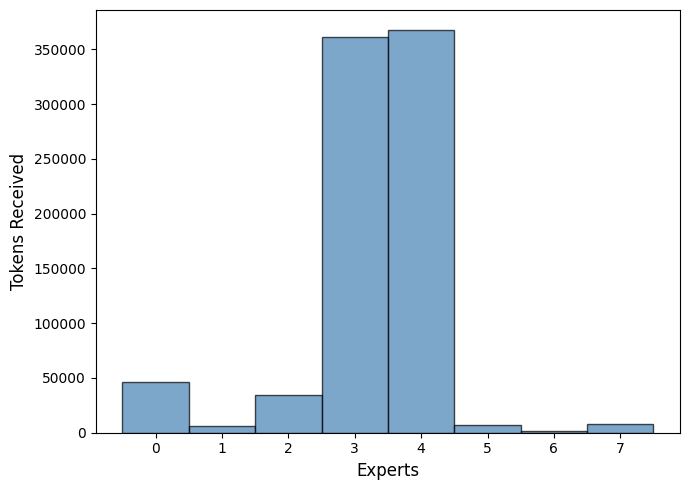
\includegraphics[width=1\linewidth]{report_images/conll/noisy_top_k.png}
  \caption{CoNLL-2003}
  \label{fig:noisy_conll}
\end{subfigure}%
\begin{subfigure}{.5\textwidth}
  \centering
  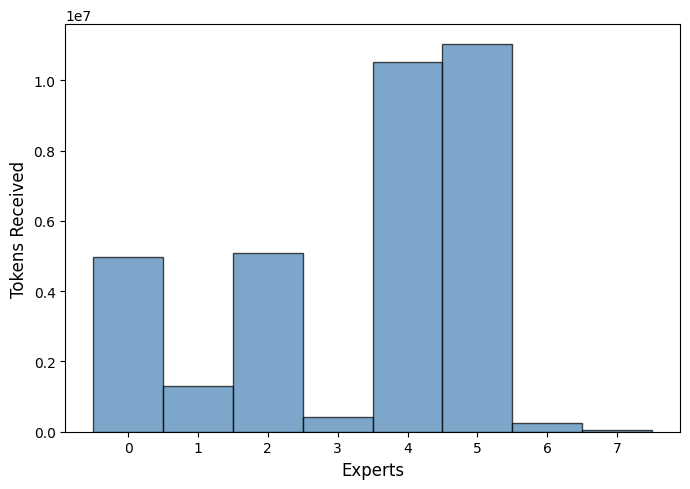
\includegraphics[width=1\linewidth]{report_images/squad/noisy_top_k.png}
  \caption{SQuAD 1.1}
  \label{fig:noisy_squad}
\end{subfigure}
\caption{Noisy Top-K Gating Expert Distributions}
\label{fig:noisy}
\end{figure}
\FloatBarrier
\noindent
The added stochasticity forced the router to use other experts. In spite of this, the model being trained on CoNLL still focused only on two experts (Fig \ref{fig:noisy_conll}). This could allude to the router not heeding much to the noise element of $H(\mathbf{x})_i$. 


\subsection{Importance Loss}
Importance of an expert relative to a batch of training examples to be the batch-wise sum of the gate values for that expert. 
\begin{equation}
\text{Importance}(\mathbf{X}) = \sum_{\mathbf{x\in X}}G(\mathbf{x})
\end{equation}
An additional loss $L_{\text{importance}}$ defined through this which encourages all the experts to have equal importance. 
\begin{equation}
L_{\text{importance}}(\mathbf{X}) = w_{\text{importance}}\cdot CV(\text{Importance}(\mathbf{X}))^2
\end{equation}
where $w_{\text{importance}}$ a hand-tuned weighing factor and 
\begin{equation}
CV(\text{Importance}(\mathbf{X})) = \frac{\sigma(\text{Importance}(\mathbf{X}))}{\mu(\text{Importance}(\mathbf{X}))+\epsilon}
\end{equation}
where $\epsilon$ is a small term added for numerical stability.

$\boldsymbol{w_{\text{importance}}=0.1}$ was being used for training.
\begin{figure}[h]
\centering
\begin{subfigure}{.5\textwidth}
  \centering
  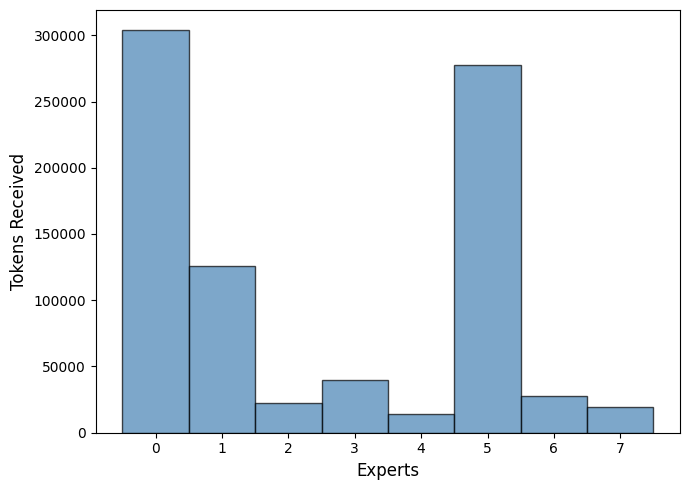
\includegraphics[width=1\linewidth]{report_images/conll/importance.png}
  \caption{CoNLL-2003}
  \label{fig:importance_conll}
\end{subfigure}%
\begin{subfigure}{.5\textwidth}
  \centering
  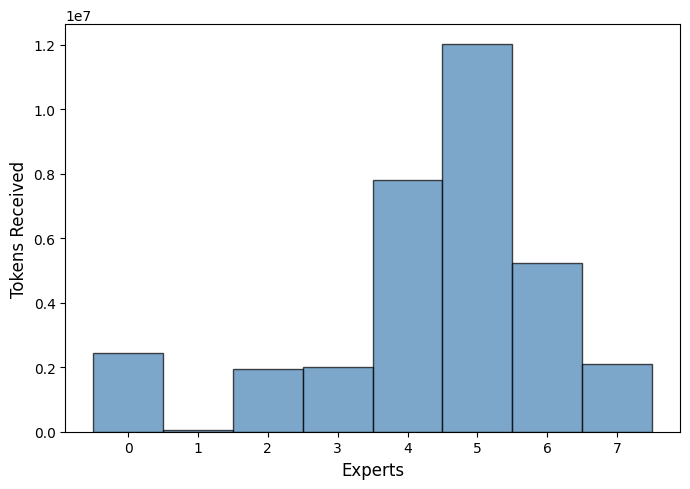
\includegraphics[width=1\linewidth]{report_images/squad/importance.png}
  \caption{SQuAD 1.1}
  \label{fig:importance_squad}
\end{subfigure}
\caption{Top-K Mask Gating with $L_{\text{importance}}$ Expert Distributions}
\label{fig:importance}
\end{figure}
\FloatBarrier
\noindent
Explicitly penalizing the narrowing of expert selection of router of the model trained on the CoNLL dataset finally forced it to select other experts for its tasks (Fig \ref{fig:importance_conll}). The SQuAD model still tried to decrease its loss by maximising use of most of the resources available to it (Fig \ref{fig:importance_squad}).

\subsection{Load Loss}
The load loss is a mechanism designed to ensure a balanced distribution of workload among the various experts in noisy top-k gating.
\begin{equation}
P(\mathbf{x}, i) = \Pr\left( (\mathbf{x} \cdot \mathbf{W}_g)_i + X \cdot \text{Softplus}((\mathbf{x} \cdot \mathbf{W}_{\text{noise}})_i) > \text{kth\_excluding}(H(\mathbf{x}), k, i)\right)
\end{equation}
where $\text{kth\_excluding}(v, k, i)$ means the $k$-th highest component of $v$, excluding component $i$ and $X\sim\mathcal{N}(0,1)$ is clearly a random variable. So the given probability can be evaluated to
\begin{equation}
P(\mathbf{x}, i) = \Phi\left( \frac{ (\mathbf{x} \cdot \mathbf{W}_g)_i - \text{kth\_excluding}(H(\mathbf{x}), k, i) }{\text{Softplus}((\mathbf{x} \cdot \mathbf{W}_{\text{noise}})_i)} \right)
\end{equation}
where $\Phi$ is the CDF of the standard normal distribution. Therefore we can define load as
\begin{equation}
\text{Load}(\mathbf{X})_i = \sum_{\mathbf{x} \in \mathbf{X}} P(\mathbf{x}, i)
\end{equation}
Finally, load loss can be defined as
\begin{equation}
L_{\text{Load}}(\mathbf{X}) = w_{\text{load}} \cdot CV(\text{Load}(\mathbf{X}))^2
\end{equation}
where $w_{\text{load}}$ a hand-tuned weighing factor and 
\begin{equation}
CV(\text{Load}(\mathbf{X})) = \frac{\sigma(\text{Load}(\mathbf{X}))}{\mu(\text{Load}(\mathbf{X}))+\epsilon}
\end{equation}
where $\epsilon$ is a small term added for numerical stability.

$\boldsymbol{w_{\text{load}}=0.1}$ was being used for training.
\begin{figure}[h]
\centering
\begin{subfigure}{.5\textwidth}
  \centering
  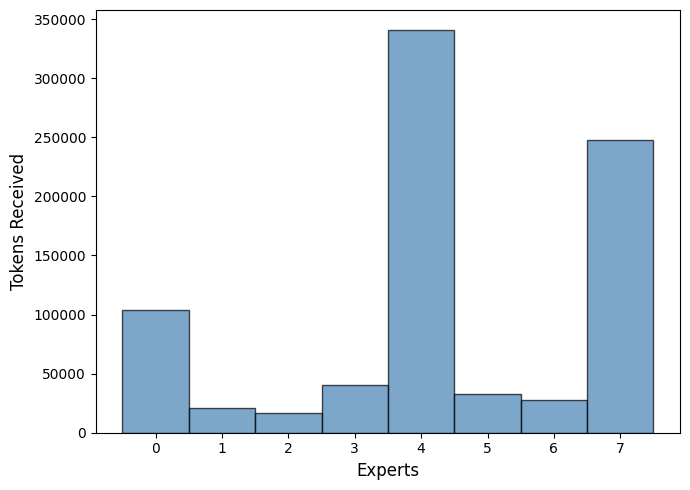
\includegraphics[width=1\linewidth]{report_images/conll/load.png}
  \caption{CoNLL-2003}
  \label{fig:load_conll}
\end{subfigure}%
\begin{subfigure}{.5\textwidth}
  \centering
  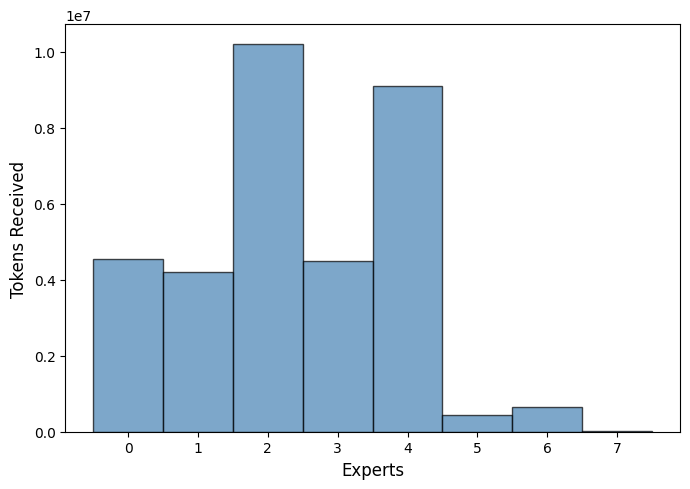
\includegraphics[width=1\linewidth]{report_images/squad/load.png}
  \caption{SQuAD 1.1}
  \label{fig:load_squad}
\end{subfigure}
\caption{Top-K Mask Gating with $L_{\text{load}}$ Expert Distributions}
\label{fig:load}
\end{figure}
\FloatBarrier
\noindent
The noisy top-k router of the CoNLL model finally budged after being forced to balance its loads (Fig \ref{fig:load_conll}). The SQuAD model spreads the use of its experts with the load loss (Fig \ref{fig:load_squad}) as compared to before.

%%%%%%%%%%%%%%%%%%%%%%%%%%%%%%%%%%%%%%%%%%%%%%%
\section{Conclusion}
With the gating strategies covered above, we can clearly see that the models being trained on \textbf{CoNLL didn't diverge from two experts} - most likely due to the fact that it \textbf{only need those two experts} to get good results on the dataset. On the other hand, the models being trained on \textbf{SQuAD} tried to \textbf{maximise the use of the resources} available to it since they were getting quite high log-likelihoods as loss (Fig \ref{fig: squad_losses}).

\end{document}





